\chapter{Implementation of the application}\label{sect:implementation}

\tab As an application we have chosen to implement a web application which can switch the DB at run time. The application will be focusing on the public transport sector, basically it will be able to display where every car is located on a map. In order to implement this we will use Java for the implementation of the back end, Spring Data which is part of Spring Framework for the implementation of the persistence layer and for the graphical user interface we will use Primefaces, which is a Java library meant to implement the graphical user interface and it is based on JSF technology.

\tab The data base layer is implemented using Sping Data because of the flexibility, we will need to switch the database from SQL to NoSQL based on a setting or something. Spring Framework is composed out of multiple modules and one module of interest is Spring Data JPA which handles the persistence layer for us, we just need to plug in some configurations, such as host and port of data base and credentials for the data base connection such as user name and port. From the module Spring Data JPA we are going to use two or more 'sub modules', one for the SQL persistence and another one for the NoSQL persistence. The first sub module is called 'spring-boot-starter-data-jpa' and it will be used as a dependency in our project for the SQL persistence and the other sub module is called spring-boot-starter-data-redis' and it will be used as a dependency as well in our project for the NoSQL persistence. For the data base switch we will implement a strategy pattern which will load the data base that we want for the current run based on a property that will be defined in a configuration file.

\tab The application will receive as an input a set of data from GPS sensors which then will be stored into a DB and then the data will be retrieved by the user in order to see where the public transport car is. In the screenshot below you can see that we managed to simulate some GPS coordinates and then generated a map with pins, representing positions on the map.

\begin{center}
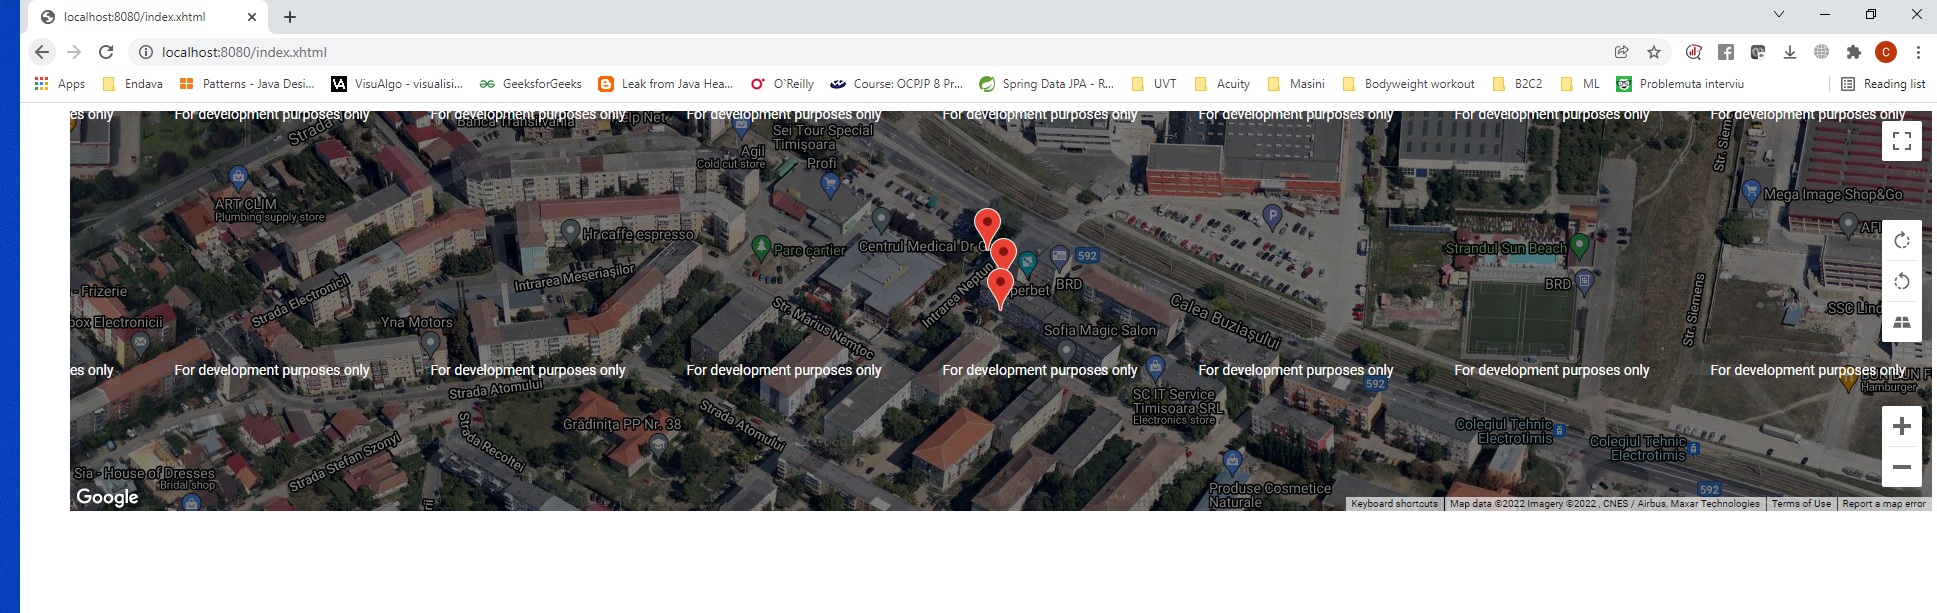
\includegraphics[width=400pt]{first screenshot.PNG} 
\end{center}

\section {Designing an application which can be able to switch database at runtime}
\tab Designing an application which can be able to switch database at runtime ...
\newline

\section {Performance comparison between SQL and NoSQL}
\tab Details about Performance comparison between SQL and NoSQL ...
\newline


\section {What and why?}
\tab Details about What and why? ...
\newline